\documentclass[12pt]{article}
\usepackage[english]{babel}
\usepackage[utf8]{inputenc}

%% Pointer to 'default' preamble, other reusable files
% pacakages and definitions

\usepackage{geometry}
\geometry{
	letterpaper, 
	portrait, 
	top=.75in,
	left=.8in,
	right=.75in,
	bottom=.5in		} 	% Page Margins
	
%% additional packages for nice things
\usepackage{amsmath} 	% for most math
\usepackage{commath} 	% for abs
\usepackage{lastpage}	% for page count
\usepackage{amssymb} 	% for therefore
\usepackage{graphicx} 	% for image handling
\usepackage{wrapfig} 	% wrap figures
\usepackage[none]{hyphenat} % for no hyphenations
\usepackage{array} 		% for >{} column characterisctis
\usepackage{physics} 	% for easier derivative \dv....
\usepackage{tikz} 		% for graphic@!
\usepackage{circuitikz} % for circuits!
\usetikzlibrary{arrows.meta} % for loads
\usepackage[thicklines]{cancel}	% for cancels
\usepackage{xcolor}		% for color cancels
\usepackage[per-mode=fraction]{siunitx} % for si units and num
\sisetup{group-separator = {,}, group-minimum-digits = 3} % additional si unit table functionality

\usepackage{fancyhdr} 	% for header
\usepackage{comment}	% for ability to comment out large sections
\usepackage{multicol}	% for multiple columns using multicols
\usepackage[framed,numbered]{matlab-prettifier} % matlab sytle listing
\usepackage{marvosym} 	% for boltsymbol lightning
\usepackage{pdflscape} 	% for various landscape pages in portrait docs.
%\usepackage{float}
\usepackage{fancyvrb}	% for Verbatim (a tab respecting verbatim)
\usepackage{enumitem}	% for [resume] functionality of enumerate
\usepackage{spreadtab} 	% for using formulas in tables}
\usepackage{numprint}	% for number format in spread tab
\usepackage{subcaption} % for subfigures with captions
\usepackage[normalem]{ulem} % for strike through sout

% for row colors in tables....
\usepackage{color, colortbl}
\definecolor{G1}{gray}{0.9}
\definecolor{G2}{rgb}{1,0.88,1}%{gray}{0.6}
\definecolor{G3}{rgb}{0.88,1,1}

% For table formatting
\usepackage{booktabs}
\renewcommand{\arraystretch}{1.2}
\usepackage{floatrow}
\floatsetup[table]{capposition=top} % put table captions on top of tables

% Caption formating footnotesize ~ 10 pt in a 12 pt document
\usepackage[font={small}]{caption}

%% package config 
\sisetup{output-exponent-marker=\ensuremath{\mathrm{E}}} % for engineer E
\renewcommand{\CancelColor}{\color{red}}	% for color cancels
\lstset{aboveskip=2pt,belowskip=2pt} % for more compact table
%\arraycolsep=1.4pt\def
\setlength{\parindent}{0cm} % Remove indentation from paragraphs
\setlength{\columnsep}{0.5cm}
\lstset{
	style      = Matlab-editor,
	basicstyle = \ttfamily\footnotesize, % if you want to use Courier - not really used?
}
\renewcommand*{\pd}[3][]{\ensuremath{\dfrac{\partial^{#1} #2}{\partial #3}}} % for larger pd fracs
\renewcommand{\real}[1]{\mathbb{R}\left\{ #1 \right\}}	% for REAL symbol
\newcommand{\imag}[1]{\mathbb{I}\left\{ #1 \right\}}	% for IMAG symbol
\definecolor{m}{rgb}{1,0,1}	% for MATLAB matching magenta
	
%% custom macros
\newcommand\numberthis{\addtocounter{equation}{1}\tag{\theequation}} % for simple \numberthis command

\newcommand{\equal}{=} % so circuitikz can have an = in the labels
\newcolumntype{L}[1]{>{\raggedright\let\newline\\\arraybackslash\hspace{0pt}}m{#1}}
\newcolumntype{C}[1]{>{\centering\let\newline\\\arraybackslash\hspace{0pt}}m{#1}}
\newcolumntype{R}[1]{>{\raggedleft\let\newline\\\arraybackslash\hspace{0pt}}m{#1}}

%% Header
\pagestyle{fancy} % for header stuffs
\fancyhf{}
% spacing
\headheight 29 pt
\headsep 6 pt
%%% custom commands for nicer units
\newcommand{\mw}{\ensuremath{\text{ MW}}}
\newcommand{\hz}{\ensuremath{\text{ Hz}}}
\newcommand{\pu}{\ensuremath{\text{ Pu}}}
\newcommand{\sbase}{\ensuremath{\text{S}_{\text{Base}}}}
\newcommand{\fbase}{\ensuremath{f_{\text{Base}}}}
\newcommand{\mbase}[1]{\ensuremath{\text{M}_{\text{Base}_{#1}}}}
\newcommand{\hsys}{\ensuremath{\text{ H}_{\text{sys}}}}


%% Header
\rhead{Thad Haines \\ Page \thepage\ of \pageref{LastPage}}
\chead{Mini WECC Delay Scenario \\ 01-24-20}
\lhead{Research \\ }

%\usepackage{graphicx}
%\graphicspath{ {figures/} }
%\newcommand{\caseName}{ }

\begin{document}
\paragraph{Scenario: } 
Using the three area mini WECC system, Figure \ref{fig: miniWECC}, a 200 MW step event was simulated in the South (Area 3) at $t=2$.
Initially, $\approx$2545 MW are being sent South over the COI.
MW flows from Bus 89 to Area 3 are compared for both a 200 MW load step and a -200 MW generation step.
Additionally, $\omega$ input to three generators in the North (Area 1) were delayed by 40 seconds.
The combined MW capacity of the generators with delay is 16,900 MW, which is $\approx$40\% of the area governed capacity or $\approx$13.8\% of the total system governed capacity.

% six machine system
\begin{figure}[!ht]
	\centering
	\footnotesize
	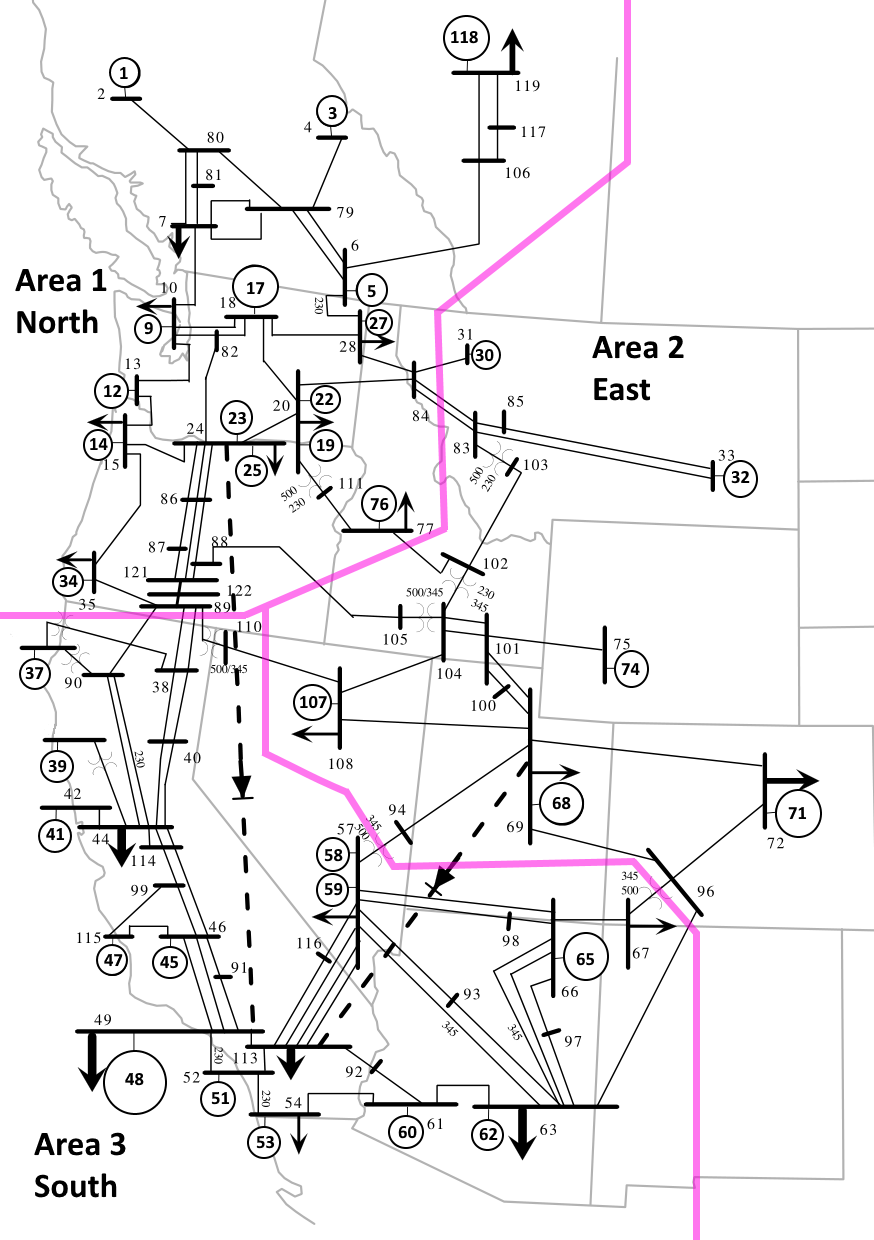
\includegraphics[height=6.5 in]{../../../paint.net/miniWECC_split/miniWECC_split03}
	\caption{Three Area Mini WECC system.}
	\label{fig: miniWECC}
\end{figure}

\paragraph{Results:} 
In a system of this size,
delaying governor response has negligible effect on frequency nadir, however, the delay introduces a second frequency perturbance roughly 40 seconds after the first frequency event that leads to a slight MW flow over response from $t=1$ to $t= 1.5$ minutes.
Additionally, while the frequency response appears essentially the same between load step and generation step cases, MW flow is approximately 25 MW larger during a load step.

\pagebreak
\paragraph{Base Case - Load Step +200 MW} \ \\

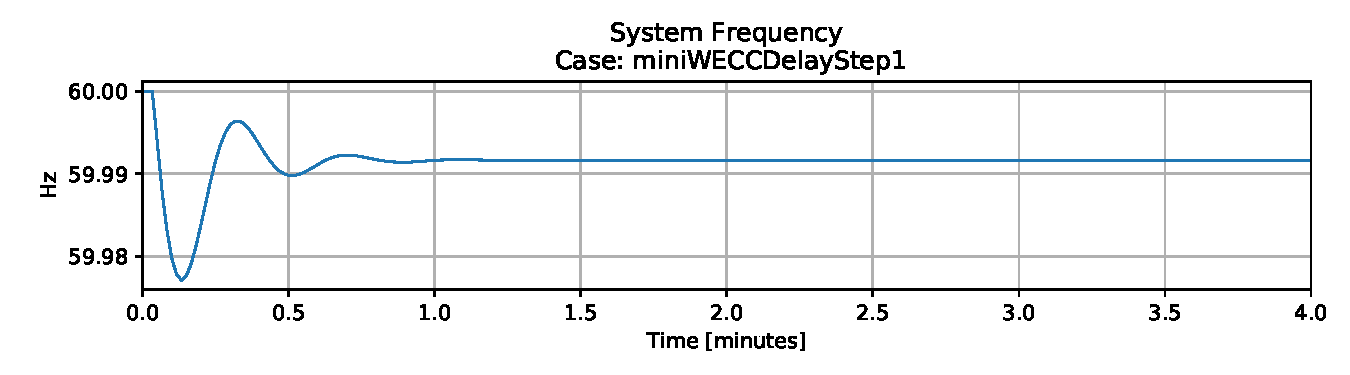
\includegraphics[width=\linewidth]{figures/miniWECCDelayStep1Freq}

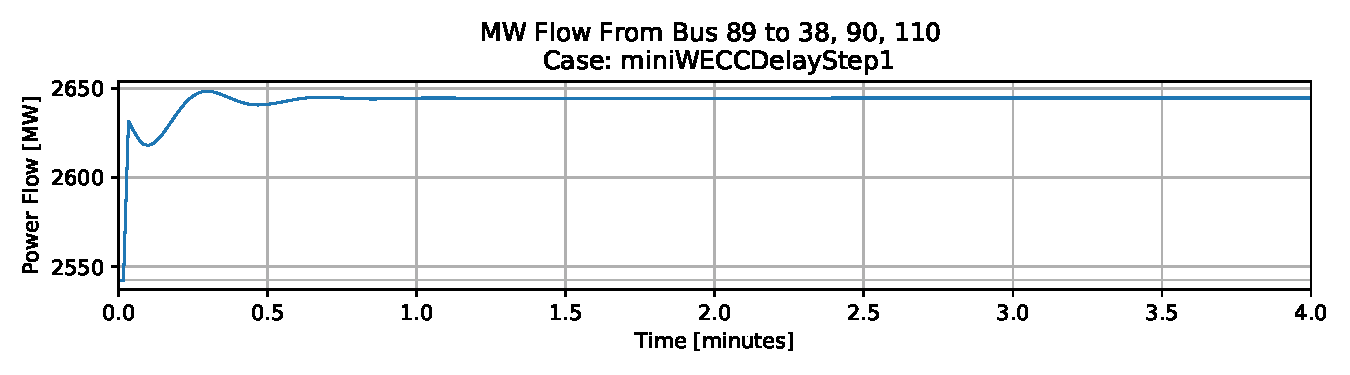
\includegraphics[width=\linewidth]{figures/miniWECCDelayStep1MWflow89to38-90-110}

\paragraph{Delay Case - Load Step +200 MW} \ \\
Input $\omega$ was delayed by 40 seconds.

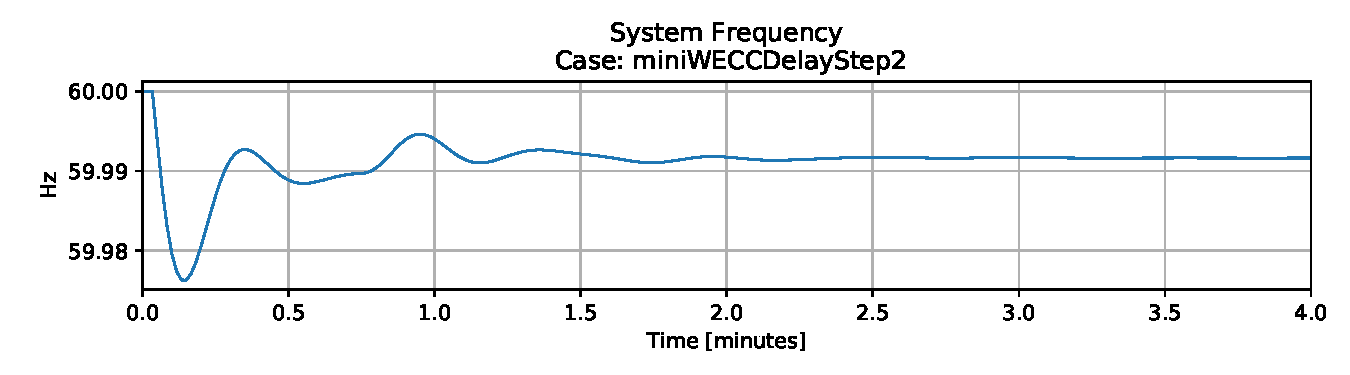
\includegraphics[width=\linewidth]{figures/miniWECCDelayStep2Freq}


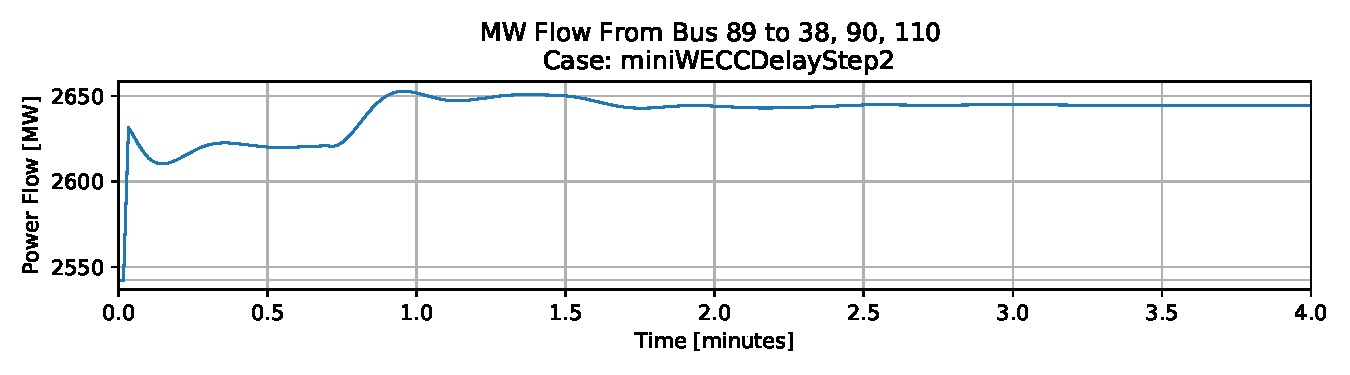
\includegraphics[width=\linewidth]{figures/miniWECCDelayStep2MWflow89to38-90-110}

\pagebreak

\paragraph{Base Case - Generation step -200 MW}\ \\

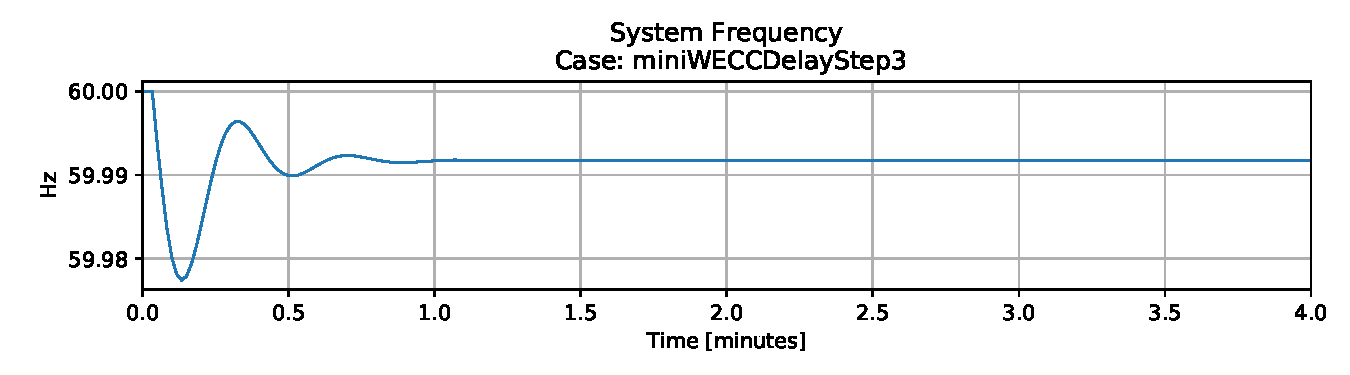
\includegraphics[width=\linewidth]{figures/miniWECCDelayStep3Freq}

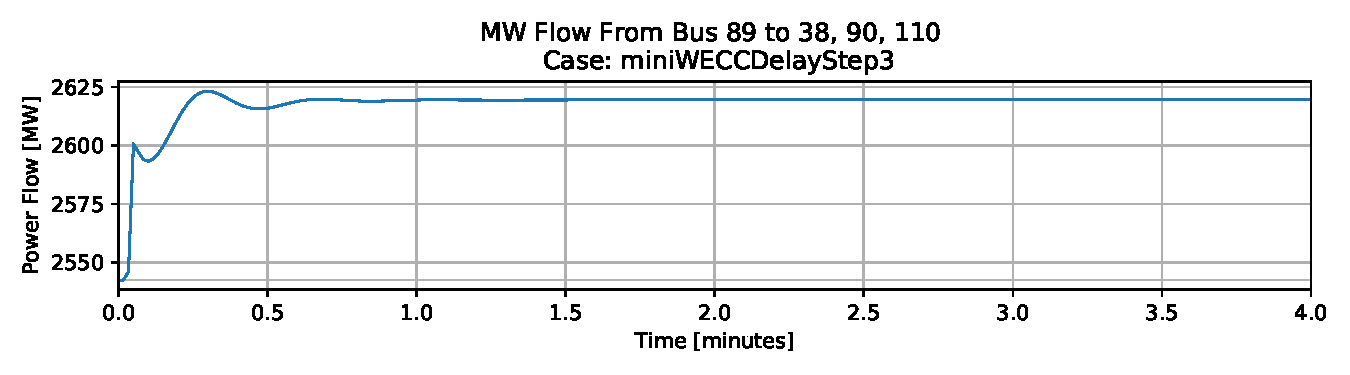
\includegraphics[width=\linewidth]{figures/miniWECCDelayStep3MWflow89to38-90-110}

\paragraph{Delay Case - Generation step -200 MW} \ \\
Input $ \omega$ was delayed by 40 seconds.

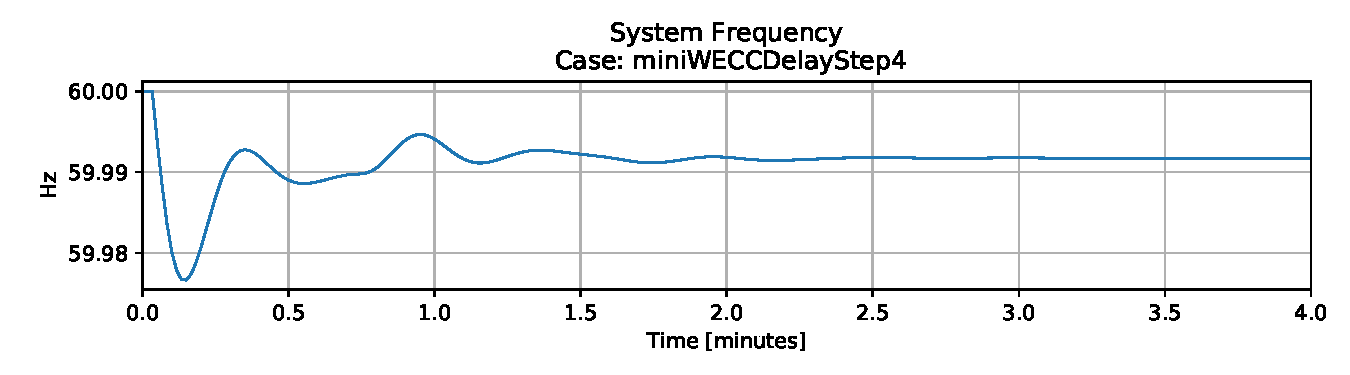
\includegraphics[width=\linewidth]{figures/miniWECCDelayStep4Freq}


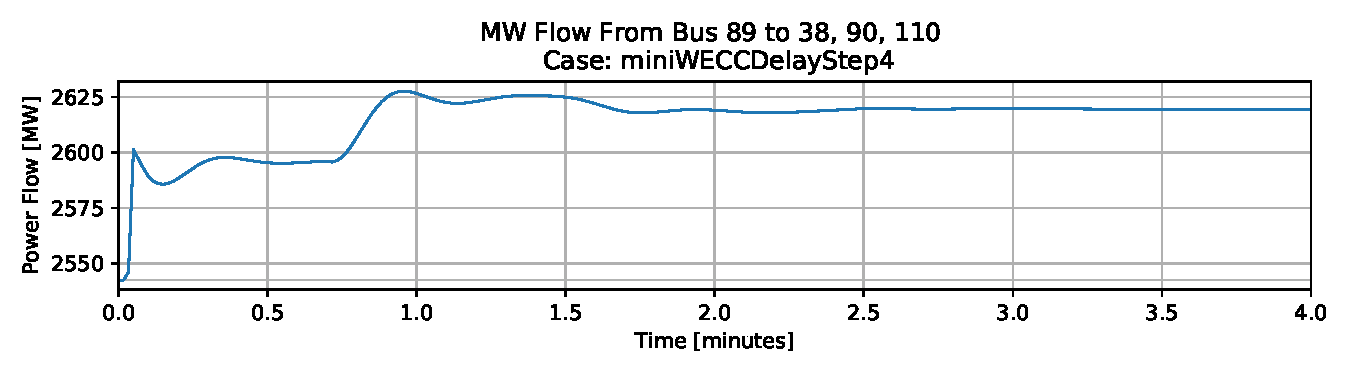
\includegraphics[width=\linewidth]{figures/miniWECCDelayStep4MWflow89to38-90-110}
\end{document}